%%%%%%%%%%%%
%
% $Autor: Wings $
% $Datum: 2019-03-05 08:03:15Z $
% $Pfad: Sketch.tex $
% $Version: 4250 $
% !TeX spellcheck = en_GB/de_DE
% !TeX encoding = utf8
% !TeX root = manual 
% !TeX TXS-program:bibliography = txs:///biber
%
%%%%%%%%%%%%

\chapter{Skizze}
Jetzt kommt ein Beispielbild mit Tikz \\
\\
	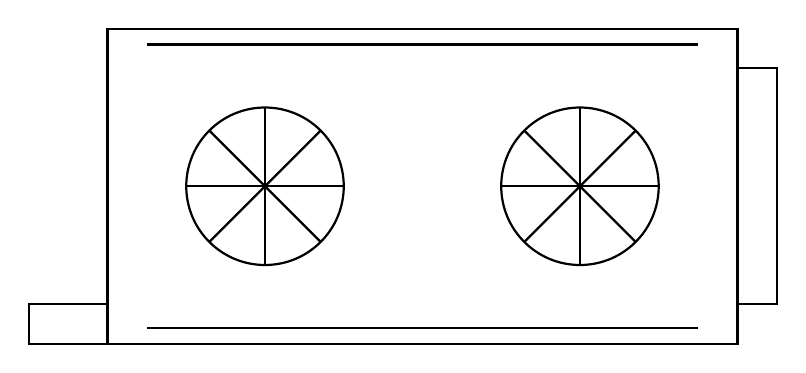
\begin{tikzpicture}
		% Gehäuse der Grafikkarte
		\draw[thick] (0,0) rectangle (8,4);
		
		% PCIe-Anschluss
		\draw[thick] (0,0) -- (-1,0) -- (-1,0.5) -- (0,0.5);
		
		% Lüfter 1
		\draw[thick] (2,2) circle (1);
		\foreach \angle in {0,45,...,315}
		\draw[thick] (2,2) --++ (\angle:1);
		
		% Lüfter 2
		\draw[thick] (6,2) circle (1);
		\foreach \angle in {0,45,...,315}
		\draw[thick] (6,2) --++ (\angle:1);
		
		% Kühler-Design
		\draw[thick] (0.5,3.8) -- (7.5,3.8);
		\draw[thick] (0.5,0.2) -- (7.5,0.2);
		
		% Steckblende
		\draw[thick] (8,3.5) -- (8.5,3.5) -- (8.5,0.5) -- (8,0.5);
	\end{tikzpicture}


